\documentclass{article}
\usepackage{listings}
\usepackage{amsmath, amsthm, amssymb, amsfonts}
\usepackage{thmtools}
\usepackage{graphicx}
\usepackage{setspace}
\usepackage{geometry}
\usepackage{float}
\usepackage{hyperref}
\usepackage[utf8]{inputenc}
\usepackage[english]{babel}
\usepackage{framed}
\usepackage[dvipsnames]{xcolor}
\usepackage{tcolorbox}

\colorlet{LightGray}{White!90!Periwinkle}
\colorlet{LightOrange}{Orange!15}
\colorlet{LightGreen}{Green!15}

\newcommand{\HRule}[1]{\rule{\linewidth}{#1}}


\setstretch{1.2}
\geometry{
    textheight=9in,
    textwidth=5.5in,
    top=1in,
    headheight=12pt,
    headsep=25pt,
    footskip=30pt
}

% ------------------------------------------------------------------------------

\begin{document}

% ------------------------------------------------------------------------------
% Cover Page and ToC
% ------------------------------------------------------------------------------

\title{ \normalsize \textsc{}
		\\ [2.0cm]
		\HRule{1.5pt} \\
		\LARGE \textbf{\uppercase{Documento di Note}
		\HRule{2.0pt} \\ [0.6cm] \LARGE{In questo documento vengono riportati i concetti affrontati durante lo stage presso Synclab S.r.L.} \vspace*{10\baselineskip}}
		}
\date{}
\author{\textbf{Author} \\ 
		Marco Brugin \\
		Synclab S.r.L. \\
		\today}

\maketitle
\newpage

\tableofcontents
\newpage

\section{Streaming ad eventi}
È una pratica di acquisizione dei dati in tempo reale da fonti di eventi come database, flussi di eventi; memorizando tutto ciò per un recupero futuro di tali informazioni, reagendo a flussi di eventi in tempo reale. Inoltre garantisce un flusso  continuo di info corrette nel posto giusto e  al momento giusto.
\subsection{Utilizzi}
\begin{itemize}
    \item per transazioni
    \item per servizzi IOT di vario genere
    \item monitoraggio sanitario 
    \item ovunque ci sia la necessità di trattare grandi moli di dati efficientemente
\end{itemize}
\section{Apache \textbf{Kafka}}
\textbf{Kafka} è una piattaforma open source che combina 3 funzionalità in modo da poter soddisfare i casi d'uso sopra citati:
\begin{itemize}
    \item pubblica e sottoscrive flussi di eventi, importandoli ed 	esportandoli da altri sistemi;
    \item archivia tali flussi in modo affidabile e duraturo;	
    \item elabora flussi di eventi in real time o in modo retrospettivo.
\end{itemize}
\subsection{Utilizzo}
\textbf{Kafka} opera su una architettura distribuita. Può essere distribuito e utilizzato in vari modi tra cui virtual machine e container, on-promise, o servizi cloud.

\subsection{Funzionamento}
\textbf{Kafka} nasce come sistema distribuito che opera su nodi che comunicano tramite protocollo \textbf{TCP} ad alte prestazioni. Data la sua natura distribuita implementa capacità di fault tollerance con rimpiazzo dei nodi guasti. 
\textbf{Kafka} è costituito da due componenti essenziali: server e client.
\subsubsection{Server}
\textbf{Kafka} viene eseguito come un cluster di uno o più server. Alcuni fanno da \textbf{broker}: livello di archiviazione. Altri assolvono il compito di \textbf{\textbf{Kafka} Connect}: importano e esportano i dati sotto forma di  flussi di eventi che permette di interagire con altri sistemi esistenti.
\subsubsection{Client}
Consentono di scrivere applicazioni distribuite e microservizi che leggono, scrivono ed elaborano flussi di eventi in parallelo, su larga scala e con fault tollerance anche in caso di problemi di rete o guasti della macchina.
Esitono molti client per diversi linguaggi di programmazione.
\subsection{Garanzie di funzionamento}
In \textbf{Kafka} esistono produttori e consumatori che producono e sottoscrivono eventi. 
Gli uni sono sono indipendenti l'uno dall'altro, ciò permette di raggiungere alcune delle seguenti garanzie:
\begin{itemize}
    \item \textbf{Al massimo una volta}: i messaggipossono andare persi ma mai riconsegnati. Infatti si potrebbe verificare un guasto ad un singolo broker o un errore della rete nel momento dell'invio di un messaggio. Il messaggio stesso verrà recapitato una e una sola volta.
    \item \textbf{Almeno una volta}: i mesaggi non 		vengono mai persi ma possono essere 		riconsegnati;
    \item \textbf{Una solo volta}: i messaggi non  		vanno persi e sono consegnati una 		sola volta; è la garanzia maggiormente desiderabile.
\end{itemize}
\subsection{Gestione degli eventi}
Gli eventi sono organizzati in topic o argomenti. Gli eventi possono essere letti da più consumatori. 
Un evento anche se consumato non viene eliminato, può essere impostato un timeout di mantenimento dell'evento.
I topic sono partizionati su più nodi. Tale partizionamento consente ai client di leggere e scrivere dati da/a molti broker. Quando un nuovo evento viene emesso questo si aggiunge all rispettiva partizione. Sarà \textbf{\textbf{Kafka}} a garantire che gli eventi vengano letti nell'ordine in cui sono stati scritti.
\subsection{Interfacce presentì}
\subsubsection{\textbf{Kafka} Producer}
L’interfaccia Producer permette alle applicazioni di inviare i flussi di dati ai broker di un cluster di Apache per categorizzarli e salvarli (nei topic già citati).
\subsubsection{\textbf{Kafka} Consumer}
L’interfaccia Consumer consente ai consumatori di Apache \textbf{Kafka} di  ricevere l’accesso ai dati, salvati nei topic di un cluster.
 \subsubsection{\textbf{Kafka} Connect}
    L’interfaccia Connect  consente di impostare produttori e consumatori riutilizzabili che collegano i topic di \textbf{Kafka} con le applicazioni o le banche dati esistenti.
\subsection{Replicas}
Con il termine di \textbf{Kafka Replication} significa disporre di più copie dei dati, distribuite su più server/broker.
Ciò aiuta a mantenere alti livelli di disponibilità in caso di guasto. \\Le repliche sono permesse  a livello di partizione. kafka ne designa una chimata leader mentre le altre  sono partizioni follower o \textbf{in-sync}. Il numero totale di repliche incluso il leader costituisce il fattore di replicazione.
Il leader è responsabile della ricezione e dell'invio dei dati, per quella partizione.
Per mantenere questi cluster e gli argomenti/partizioni all'interno, Kafka ha un servizio centralizzato chiamato \textbf{Zookeeper}.

\subsection{Retention}
Con \textbf{Retention} in \textbf{Kafka} si intende la possibilità di controllare la dimensione dei registri degli argomenti ed evitare di superare le dimensioni del disco esistente.\\La conservazione può essere configurata o controllata in base alla dimensione dei log o in base alla durata configurata.
Tale configurazione può essere impostata a grana fine o a grana grossa per ogni argomento o per tutti gli argomenti.\\
\subsubsection{Retention basata sul tempo}
Una volta raggiunto il tempo di conservazione configurato per il segmento, questo viene contrassegnato per l'eliminazione o la compattazione in base al criterio di pulizia configurato. Il periodo di conservazione predefinito per i segmenti è di 7 giorni.
In ordine di importanza i parametri configurabili per la    \textbf{Retention} basata sul tempo sono in ordine di importanza e valutazione:
\begin{enumerate}
    \item log.retention.ms;
    \item log.retention.minutes;
    \item log.retention.hours.
\end{enumerate}
Nel momento in cui un parametro di livello di priorità superiore non è impostato si segue ciò che indica quello di livello appena inferiore.
\subsubsection{Retention basata sulle dimensione}
In questo caso si va 
configurare la dimensione massima di una struttura di dati di registro per una partizione di argomento. Una volta che la dimensione del registro raggiunge questa dimensione, inizia a rimuovere i segmenti dalla sua fine.
\\
In ordine di importanza i parametri configurabili per la    \textbf{Retention} basata dimensione sono in ordine di importanza e valutazione:
\begin{enumerate}
    \item log.segment.bytes: la dimensione massima di un singolo file di registro;
    \item log.retention.check.interval.ms: la frequenza in millisecondi con cui la pulizia del registro verifica se un registro è idoneo per l'eliminazione;
    \item log.segment.delete.delay.ms: la quantità di tempo da attendere prima di eliminare un file dal file system.
\end{enumerate}
\subsection{Zookeeper}
\textbf{Zookeeper} si occupa della sincronizzazione tra i cluster distribuiti e ne gestisce le configurazioni, il controllo e la denominazione.\\
Il protocollo \textbf{Zookeeper Atomic Broadcast (ZAB)} è il cervello dell'intero sistema.\\
Ogni replica o nodo invia a intervalli regolari un messaggio \textit{ Keep-Alive} a Zookeeper, informando così \textbf{Zookeeper} che è vivo e funzionante. \\
Se ebtro un tempo prestabilito il messaggio non viene ricevuto si presume che il nodo sia morto e se era un leadere se ne elegge un altro.\\
\textbf{Zookeeper} permette di definire dei parametri che consentono di capire quando un nodo è guasto e quanto i nodi follower sono in ritardo rispetto al leader.\\
Il parametro zookeeper.session.timeout.ms millisecondi è impostato su 6000 per impostazione predefinita: indica che ,se il leader non riceve l'evento \textit{ Keep-Alive} entro quel periodo temporale, detiene che quel nodo sia morto.\\
Il parametro replica.lag.max.messages, decide la differenza consentita tra \textbf{Replica's Offset
}e \textbf{Leader's Offset}. Se questa differenza è maggiore di replica.lag.max.message-1, il nodo viene considerato in ritardo e viene rimosso dall'elenco dei nodi in sincronizzazione dal leader. \\
Tutti i nodi che sono attivi e sincronizzati formano l' \textbf{In-Sync Replica Set}(\textbf{ISR}).\\
Ora, se tutti i nodi in sincronizzazione hanno applicato un messaggio ai rispettivi log, questo messaggio viene considerato confermato e quindi inviato ai consumatori. In questo modo, \textbf{Kafka} garantisce che un messaggio di cui è stato eseguito il commit non andrà perso, purché sia presente almeno una replica attiva e sincronizzata, in ogni momento.\\
Un nodo non sincronizzato può ricongiungersi all'\textbf{ISR} se può risincronizzarsi completamente di nuovo, anche se ha perso alcuni dati a causa del suo arresto anomalo.
\subsection{Kraft}
\textbf{Apache Kafka Raft (KRaft)} è il protocollo di consenso introdotto per rimuovere la dipendenza di \textbf{Apache Kafka} da \textbf{ZooKeeper} per la gestione dei metadati. Ciò semplifica enormemente l'architettura di \textbf{Kafka} consolidando la responsabilità dei metadati all'interno di \textbf{Kafka} stesso, anziché suddividerla tra due diversi sistemi: \textbf{ZooKeeper e Kafka}.\\
\textbf{KRaft} utilizza un modello di archiviazione di origine evento che garantisce che le macchine a stati interni possano sempre essere ricreate accuratamente. Il registro eventi utilizzato per archiviare questo stato
 viene periodicamente abbreviato da istantanee per garantire che il registro non possa crescere all'infinito.\\ Gli altri nodi all'interno del quorum seguono il leader  rispondendo agli eventi che crea e memorizza nel suo registro. Pertanto, se un nodo si ferma a causa di un evento di partizionamento, ad esempio, può recuperare rapidamente eventuali eventi persi accedendo al registro quando si ricongiunge. \\
 La natura basata sugli eventi del protocollo KRaft significa che, a differenza del leader basato su ZooKeeper, il leader del quorum non ha bisogno di caricare lo stato da ZooKeeper prima che diventi attivo. Quando la leadership cambia, il nuovo leader attivo ha già tutti i record di metadati impegnati in memoria. Inoltre, lo stesso meccanismo guidato dagli eventi utilizzato nel protocollo KRaft viene utilizzato per tenere traccia dei metadati nel cluster. 
\subsection{Casi d'uso}
\subsubsection{Notifica dell'evento}
\textbf{Kafka} permette di trasmette semplicemente eventi per avvisare altri sistemi di un cambiamento nel suo dominio.
\subsubsection{Trasferimento di stato portato da eventi}
In questo utilizzo il destinatario dell'evento ottiene anche i dati di cui ha bisogno per eseguire azioni aggiuntive sui dati richiesti.
\subsubsection{Approvvigionamento di eventi}
In questo caso il sistema consente di descrivere ogni cambiamento di stato in un sistema come un evento, con ogni evento registrato in sequenza cronologica. Di conseguenza, il flusso di eventi stesso diventa la principale fonte di verità del sistema.
\subsection{Applicazioni}
\subsubsection{Messaggistica}
I broker di messaggi vengono utilizzati per disaccoppiare l'elaborazione del messaggio dal produttore dello stesso.
\textbf{Kafka} rispetto ai sistemi di messaggistica tradizionale ha una migliore velocità, partizionamento integrato e tolleranza agli errori.
L'utilizzo è basso, ma in ambiti in cui si richiede una bassa latenza, le garanzie fornite da \textbf{Kafka} sono alla pari dei tradizionali sistemi di messagistica, che lo rendono lo rendono una buona soluzione per applicazioni di elaborazione di messaggi su larga scala.

\subsubsection{Monitoraggio di siti web}
È il caso d'uso d'origine di \textbf{Kafka} , ha la caratteristica di generare un elevato volume di messaggi. Lo scopo era quello di ricostruire le attività degli utenti come insieme di eventi genrati dalle azioni dell'utente.
\subsubsection{Metrica}
Indica l'aggregazione di dati di monitoraggio provenienti da varie fonti per eseguire statistiche.
\subsubsection{Aggregazione di registri}
\textbf{Kafka} ha anche la capacità di estrarre i dati dai file di log fisici e fornisce una astrazione di tali sotto forma di flusso di messaggi. Ciò permette di garantire una più bassa latenza di elaborazione e supporto per più origini dati.
\subsubsection{Elaborazione del flusso}
È possibile andare a creare una  data-pipeline in cui i dati grezzi vengono consumati dagli argomenti di \textbf{Kafka}, aggregati, trasformati fino ad ottenere unn dato elaborato.
\subsubsection{Approvvigionamento di eventi}
È possibile utilizzare  di \textbf{Kafka} in aplicazioni cui cambiamenti di stato vengono registrati come sequenze di record in ordine temporale. \textbf{Kafka} permette il supporto per dati di registro memorizzati molto grandi tanto che lo rende un ottimo back-end di tali applicazioni. 
\subsubsection{Registro commit}
\textbf{Kafka} può fungere da sorta di log di commit esterno per un sistema distribuito. Il registro aiuta a replicare i dati tra i nodi e funge da meccanismo di risincronizzazione per consentire ai nodi non allineati di ripristinare i propri dati.

\subsection{Apache Kafka VS EDA}
L'emissione di un evento indica che qualcosa è accaduto e può essere visto come un agglomerato di dati atomico in grado di soddisfare l'evento stesso. 
\textbf{Kafka} è un sistema di streaming di eventi che gestisce un flusso continuo di eventi. Inoltre Kafka memorizza tali in modo duraturo per il successivo recupero, analisi o elaborazione in tempo reale e li inoltri a varie destinazioni secondo necessità.
\\
D'altra parte in una \textbf{EDA} (Event Driven Architecture) viene generati degli eventi che un agente acquisisce e risponde a tale evento.
per utilizzare \textbf{Kafka} in un sistema \textbf{EDA} la chiave è andare a sfruttare il disaccopiamento: invece di effetuare un polling continuo di verifica della presenza di nuovi dati, basterà ascoltare il verificarsi di un evento per agire. Inoltre grazie all'approcio sviluppato da \textbf{Kafka} un evento una volta soddisfatto non viene eliminato, ma conservato per un periodo ti tempo predeterminato, pertanto un evento potrà essere letto da più consumatori e potrà essere utilizzato per soddisfare una varietà di richieste.
\section{Even Driven Architecture}
L'\textbf{Even Driven Architecture} è un pattern archietteturale basato su eventi: degli agenti, che sono in grado di ricevere tali eventi, agiranno solo nel momento in cui questi ultimi si verificheranno. 
Una architettura basato su eventi fornisce una serie di altri vantaggi basati sul disaccopiamento tra il produttore e il consumatore dell'evento, i quali, nel momento dell'emissione di quest'ultimo non è necessario siano sincroni ma possono andare a sfruttare una comunicazione di tipo asincrona. 
\subsection{Casi d'uso}
\subsection{Integrazioni esterne}
In molti sistemi quando di verifica un evento è necessario interagire con un servizio esterno. Grazie ad una architettura ad eventi, ogni servizio sarà indipendente l'uno dall'altro, così che se un servizio riscontra problemi nella sua esecuzione gli altri non ne risenteranno, data la loro indipendenza. Inoltre anche l'aggiunta di nuovi servizi ha nessun impatto. 
\subsection{Flussi di lavoro}
L'archiettetura \textbf{EDA} può essere anche impiegata nell'orchestrazione di un flusso di lavoro; nel quale ogni servizio è responsabile di un part del flusso indipendentemente dagli altri. Il fattore chiave è andare ad eseguire il rispettivo servizio all'emissione di un determinato evento.
\subsection{Trasferimento di Stato}
La modifica di un dato è un altro caso d'uso in cui l'architettura \textbf{EDA} può essere utilizzato per segnalare in tempo reale il mutamento di un dato in una detrminata struttura dati.
\subsection{Accoppiamento temporale}
Inoltre grazie ad un' architettura \textbf{EDA} si va a rimuovere l'accopiamento temporale tra chi efettua una chiamata e chi va a risponde a quest'ultima.
\section{Middleware}
Con il termine di \textbf{Middleware} si va ad intendere un insieme di pacchetti software che molte applicazioni utilizzano per comunicare tra di loro. Il \textbf{Middleware} funge da ponte tra tecnologie differenti in modo da poterle totalmente integrare.\\
L'architettura sottostante ad un \textbf{Middleware} non è altro che una \textbf{data-pipeline} nella quale i dati passano da una applicazione in connessione all'altra. \\
La chiave di utilizzo di un \textbf{Middleware} è che fornisce disaccopiamento tra i vari stadi di una \textbf{data-pipeline}.
\section{Panoramica design pattern architetturali}
\subsection{Layered-Architecture}
È un modello architetturale basato su più livelli orrizontali, in cui ciascuno svolge un compito specifico e ha detrminata responsabilità. Sebbene il pattern in sè non indichi il numero di livelli da utilizzare, è usuale creare architetture con al più quattro livelli: presentazione, business, persistenza e database.
In tale archittetura ogni livello è del tutto separato dagli altri: le modifiche apportate ad un livello non generano cambiamenti agli altri, per questo si parla di livelli isolati.
La comunicazione tra i livelli avviene in dall'alto verso il basso e in generale attraverso livelli chiusi: il passaggio delle informazione tra due o più livelli deve attraversare tutti i livelli intermedi.

\subsection{Client-server}
Nel pattern architetturale client-server ci sono due componenti essenziali: il client, che richiede un servizio o una prestazione, e il server che la fornisce. Il client espone porte di richesta, mentre il server espone porte di servizio. In tale architettura vige un tipo di collegamento Request-Response.
Uno dei principali vantaggi di tale pattern architetturale il calcolo centralizzato dei dati.
\pagebreak
\subsection{Pipe-filter}
Il modello architetturale \textbf{Pipe-Fileter} è caraterrizzato da trasformazioni successive del flusso di dati.
\\
I dati dall'origine vengono inviati dall'origine verso le porte di input del primo filtro, dove viene eseguita la prima elaborazione, quindi il prodotto dell'elaborazione viene fornito dallì'output all'input del filtro successivo e così via.
\\
Il fattore importante in tale pattern architetturale è l'ordine con cui vengono eseguiti tali filtri.
\subsection{Broker}
Il \textbf{Broker} pattern architetturale che può essere utilizzzato per sistemi software disaccopiati e distribuiti che interagiscono tramite chiamate remote.
Il pattern è formato da tre agenti:
\begin{itemize}
    \item il client: che accede a funzionalità del server inviadno ricbhieste al broker;
    \item il server che mette a disposizione del client i propri servizzi attraverso il broker;
    \item il broker: riceve le richieste dai cleint e una volta trovato il server appropiato inoltra la richiesta e trasmette il risultato al client.
\end{itemize}
\section{Publisher-Subscriber}
Il pattern architetturale \textbf{Publisher-Subscriber} è un modello di progettazione software, utilizzato nei sistemi distribuiti, che impiegano una comunicazione asincrona tra i vari componenti.\\
Sebbene vada ad utilizare tecniche già preesistenti come la sottoscrizione e l'accodamento di messaggi, la  chiave di sucesso di tale pattern è il totale disoccopiamento delle componenti: i componenti non sono a conoscenza dell'identità e della presenza degli altri.\\
Il modello Pub-SUb è nato dalla necessità del rendere i sistemi ridimensionabili in modo dinamico.
\subsection{Architettura}
Il Pub-Sub fornisce un sistema di scambio di messaggi tra editori e sottoscrittori. Lo scambio tra questi ultimi non avviene in modo diretto tra gli agenti appena illustrati, ma viene utilizzato un intermediario che raggruppa i messaggi per argomento e fornisce disaccopiamento tra le componenti.
\subsection{Vantaggi}
\begin{itemize}
    \item \textbf{Debole accopiamento tra le componenti}: che rende il sistema più flessibile e modificabile dinamicamente;
    \item \textbf{Elevata scalabilità}: non esiste limite al numero di publisher e subscriber che possano comunicare;
    \item \textbf{Utilizzo della comunicazione ascincrona ad eventi}: non necessità della sicnrona degli attori coninvolti nella comunicazione;
    \item \textbf{Indipendente dal protocollo di comunicazione}: è integrabile con qualsiasi protocollo di comunicazione e stack tecnologico.
\end{itemize}
\section{Streaming Data pipelines}
Con il termine di 
\textbf{data-pipelines} si intende un software che consente il fluire automatico di dati da un punto ad un altro del sistema.
Di solito le origini sono molteplici e generano dati ad altissima velocità.
\\
L'architettura che sta dietro a una \textbf{data-pilenes} consente di consumare, elebaorare, archiviare dati in tempo reale, man mano che vengono generati.
Tutto ciò consente analisi e reazioni più veloci ad esigenze sorte.
\\
In generale nelle pipeline dati tradizionali estraggono, trasformano e caricano i dati prima che possano essere utilizzati.
Ma data la enorme mole di dati che le \textbf{Streaming Data pipelines} sono sottoposte, tutto ciò non è possibile.
\subsection{Architettura}
Infatti per elaborare dati in streaming provenienti da sistemi come \textbf{Kafka} è necssario creare due livelli per l'elaborazione dati: 
\begin{itemize}
    \item \textbf{Archiviazione}:
    questo livello consente la memorizzazione
    dei dati, permettendo letture e scritture a basso costo in termini computazionali mantenendo l'ordine di arrivo dei dati;
    \item \textbf{Lavorazione}: elabora e consuma i dati del livello di archiviazione andando a segnalare a quest'ultimo i dati non più necessari.
\end{itemize}
\subsection{Obiettivi}
\begin{itemize}
    \item \textbf{Scalabilità}: il volume dei dati può crescere notevolmente nel tempo quindi è necessario archiviare i dati in un \textbf{data warehouse};
    \item \textbf{Durata e consistenza}: è importante considerare che i dati letti potrebbero essere già modificati o obsoleti, quindi è fondamentale disporre di strumenti di monitoraggio del flusso dati nel tempo;
    \item \textbf{Ordinare}: l'archiettura deve essere in grado di individuare la sequenza dei dati nel flusso;
    \item 
    \textbf{Tolleranza ai guasti}: lo streaming dei dati non smettono mai di fluire da varie sorgenti e il sitema deve prevenire le interuuzioni di alcuni sorgentii;
    \item 
    \textbf{Latenza}: data l'enorme mole di dati prodotti, se questi ultimi non vengono gestiti in tempo reale perdono di rillevanza e diventano inutilizzabili.
\end{itemize}
\clearpage
\subsection{Alta affidabilità}
Il concetto di alta affidabilità è essenzialmente alla capacità di un sistema di funzionare continuamente senza guasti in un detrminato periodo di tempo.\\
Per garantire tali prestazioni in generale è necessario seguire i seguenti principi:
\begin{itemize}
    \item \textbf{Crossover affidabile}: creazione di ridondanza eseguendo l atto di passare dal componente X al componente Y senza perdere dati o influire sulle prestazioni;
    \item \textbf{Bilancio del carico}:
    tecnica attraverso  la quale si va a ridristribuire
    il carico di elaborazione da su tutte le risorse del sistema in modo tale che nessuna sia sovraccaricata;
    \item \textbf{Rillevazione e gestione automatica dei guasti}:
    i guasti devono essere visibili e i  sistemi devono disporre di un sistema deve essere provvisto di un sistema automatico in grado di gestirli autonomamente.
\end{itemize}
\section{Archietture distribuite}
Con il termine \textbf{distribuito} si va ad intendere un'architettura nella quale i componenti non si trovano su un'unica macchina ma possono cooperare attraverso una rete di comunicazione per raggiungere un detrminato obiettivo.
\\Le principali caraterristiche che si riscontrano su tale archietettura sono:
\begin{itemize}
    \item l'elaborazione non è limitata a una sola macchina;
    \item Il middleware è un'infrastruttura che supporta adeguatamente lo sviluppo e l'esecuzione di applicazioni distribuite, fornendo un buffer tra le applicazioni e la rete. Svolge il ruolo di intermediario del sistema e gestisce o supporta i diversi componenti di un sistema distribuito;
    \item le basi di un'architettura distribuita sono la  trasparenza, affidabilità e disponibilità.
\end{itemize}
\subsection{Confronto Architetture centralizzate e distribuite }
\begin{figure}[H]
    \centering
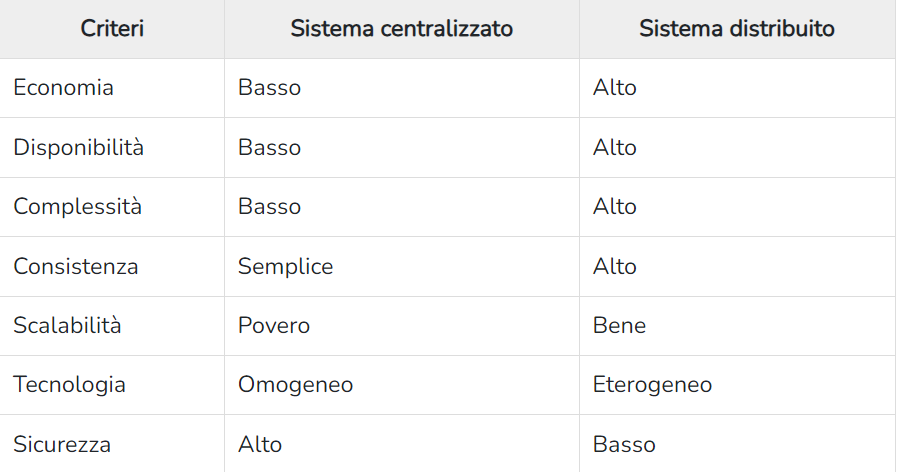
\includegraphics[scale=0.5]{images/central_vs_distribution.png}
    \caption{Confronto tra architetture centralizzate e distribuite}
    
\end{figure}
\section{Implementazione}
\subsection{Apache kafka}
Le note riportate si riferiscono ad un sistema operativo Linux dove è già stata scaricata una versione di \textbf{Apache Kafka}. I comandi devono essere eseguiti dalla cartella di installazione.
\begin{itemize}
    \item mandare in esecuzione il gestore \textbf{Zookeeper}
    \begin{lstlisting}
    bin/zookeeper-server-start.sh config/zookeeper.properties\end{lstlisting}
    \item mandare in esecuzione il \textbf{Broker}
    \begin{lstlisting}
    bin/kafka-server-start.sh config/server.properties\end{lstlisting}
    \item creare un nuovo \textbf{topic} name
   \noindent \begin{lstlisting}
   bin/kafka-topics.sh--create --topic topic--name--bootstrap-serverIP:port server \end{lstlisting}
   \item creare un \textbf{produttore} 
   \begin{lstlisting}
   bin/kafka-console-producer.sh --topic topic--name --bootstrap-server IP:port server \end{lstlisting}
   \item creare un \textbf{consumatore}
   \begin{lstlisting}
   bin/kafka-console-consumer.sh--topic topic--name--from-beginning --bootstrap-server IP:port server
   \end{lstlisting}

\end{itemize}
\section{Apache Druid}
\textbf{Apache Druid} è un database di analisi in tempo reale progettato per analisi rapide, i suoi punti di forza sono le alte prestazioni in esecuzione di query su set di dati di grandi dimensioni.
\textbf{Druid} è comunemente utilizzato come back-end del database per le GUI di applicazioni analitiche o per API altamente simultanee che richiedono aggregazioni veloci. Mostra le sue migliori prestazioni con dati orientati agli eventi.
\subsection{Caratteristiche principali}
\textbf{Druid} combina le idee provenienti da serie temporali e sistema di ricerca, \textit{data-warehouse}.
Le caratteristiche principali sono:
\begin{itemize}
    \item formato di archiviazione a colonne: utilizza una archiviazione orientata alle colonne e carica soltanto le colonne necessarie per una determinata query. Inoltre ottimizza l'archiviazione delle colonne in base al tipo di dato;
    \item sistema distribuito scalabile: le distribuzioni tipiche di Druid si estendono su cluster che vanno da decine a centinaia di server ciò permette di mantenere un tempo di latenza molto basso, al di sotto di pochi secondi;
    \item elaborazione massicciamente parallela: le query vengono elaborate in parallello sull'intero cluster;
    \item injection in tempo reale o batch: \textbf{Druid} è in grado di elaborare sia dati in tempo reale che in batch, i dati acquisiti sono immediatamente disponibili per le successive interrogazioni;
    \item è dotato di un sistema di autobilanciamento e auto individuazione dei guasti:il cluster Druid si riequilibra automaticamente in background senza tempi di inattività, inoltre se un server \textbf{Druid} si guasta, il sistema instrada automaticamente i dati intorno al danno fino alla risoluzione, infatti \textbf{Druid} è progettato per funzionare senza tempi di inattività;
    \item l'architettura nativa del cloud è tollerante ai guasti: \textbf{Druid} archivia in modo sicuro una copia dei tuoi dati in un archivio profondo (in genere su su fyle system o sul cloud), tali dati saranno accessibili semopre anche nel momento in cui i server falliscano; ciò permette l'esecuzione di query anche nei momenti di ripristino.
    \item Indici per filtraggio rapido: \textbf{Druid} utilizza indici bitmap compressi per creare indici che consentano il filtraggio rapido e la ricerca su più colonne;
    \item Partizionamento basato sul tempo: \textbf{Druid} prima suddivide i dati in base al tempo, è possibile in ogni caso aggiungere altri tipi di filtri;
   \item  Algoritmi approssimati:
   \textbf{Druid} permette l'utilizzo di algoritmi offrono un utilizzo limitato della memoria e sono spesso sostanzialmente più veloci dei calcoli esatti, dove sono richiesti conteggi più esatti \textbf{Druid} offre pure questa funzionalità.
   \item Riepilogo automatico al momento dell'acquisizione: \textbf{Druid} supporta facoltativamente il riepilogo dei dati al momento dell'acquisizione.
\end{itemize}

\subsection{Funzionamento}
\subsubsection{DistribuzioniSu singolo nodo}
\textbf{Apache Druid} include molteplici configurazioni su singola macchina si trattano di distribuzioni oramai poco utilizzate.
\\
Esistono confivgurazioni molto piccole pensate per macchine con poca \textbf{CPU} e \textbf{memoria}, pensate per ambienti con risorse limitate, come i piccoli contenitori \textit{Docker}.
\subsubsection{Distribuzione in cluster}
\textbf{Apache Druid} è progettato per essere distribuito come cluster scalabile e con tolleranza ai guasti.\\
In generale è consigliato andare a creare un cluster che ospita: 
\begin{itemize}
    \item i server principali (Coordinator e Overlord): sono responsabili della gestione dei metadati e delle esigenze di coordinamento del  cluster, possono essere collocati insieme sullo stesso server;
    \item i server dati (Historicals e MiddleManager):
    per gestire i dati effettivi nel tuo cluster,traggono grandi vantaggi da CPU, RAM e SSD;
    \item i server di interrogazione:
    i \textbf{Druid Broker} accettano le richieste e le distribuiscono al resto del cluster, facoltativamente, mantengono una cache delle query in memoria.
\end{itemize}

\section{Test}
\subsection{High AVaibility}
Per andare a testare l'alta affidabilità, si è andati a creare un cluster di nodi formato da: 1 nodo Zookeeper, 3 nodi broker (Kafka1, Kafka2,Kafka3) e si è andati ad istanziare un produttore e consumatore collegati al broker Kafka1. Ora per testare l'alta affidabilità basta simulare un malfunzionamento e verificare se i messaggi che il broker Kafka1 non è riuscito ad inviare al consumatore sono accessibili attraverso i server Kafka2 e Kafka3. 
\subsection{Svolgimento}


\subsection{verifing to connect with an another host}
\bibliographystyle{IEEEtran}
\bibliography{https://Kafka.apache.org/documentation/}
\bibliography{https://ably.com/topic/pub-sub#the-pub-sub-model-explained}
\bibliography{https://kafka.apache.org/quickstart}

\end{document}
